
\chapter{Case Study: Preventing Accuracy Regressions in Forecasting Frameworks}
\label{cha:crayon_case_study}
This Chapter investigates how to use the statistical reproducibility of Crayon benchmarks to protect forcasting libraries against accuracy regressions. Specifically, how the \textit{benchmarking} and \textit{verify} functions in Crayon can be used to detect accuracy regression through automated tests. The DeepAREstimator of Gluon-TS will be the focal point of this investigation since it suffered a accuracy regression, which has now been resolved. Thus, distributions can be collected both before, during and after a regression to showcase how these regressions can be detected and how it can be detected when they are resolved.

The DeepAREstimator in Gluon-TS suffered a accuracy regression, between the 7th of May 2020 until 9th of July 2020 for certain values of the \textit{distr\_output} hyperparameter was used. The issue arised due to a change in the way that the \textit{gluonts.distribution.NegativeBinomialOutput} was calculated. The issue was not detected until the 15 June 2020, However, the root cause of the issue was not discovered until the 2nd of July after which the bug was patched within a week on the 9th of July \cite{gluonts_deepar_bugged, gluonts_deepar_bugged_found, gluonts_deepar_patched}. In this case, the time required to detect and resolve the issue was close to two months.

To detect accuracy regression with Crayon, a reference benchmark is required to serve as a ground-truth of the expected performance for an algorithm. When new changes to algorithms or their dependencies happen, a new benchmark should be executed with these changes. These two benchmarks can then be verified using the \textit{crayon.verify} function. If they pass the checks, no accuracy regression has occurred and if the checks failed it indicates that an accuracy regression has occured. When the accuracy regression is fixed a new benchmark can be run as a post-fix benchmark. This post-fix benchmark can be verified towards the ground-truth benchmark to verify if the accuracy is back at the original levels. If a change in accuracy is expected the post-fix benchmark can be used as the new ground-truth for future tests. An overview of this method is shown in Figure \ref{fig:crayon_as_test}. This method is designed to easily be integrated into existing testing workflows.

\begin{figure}[h]
  \centering
  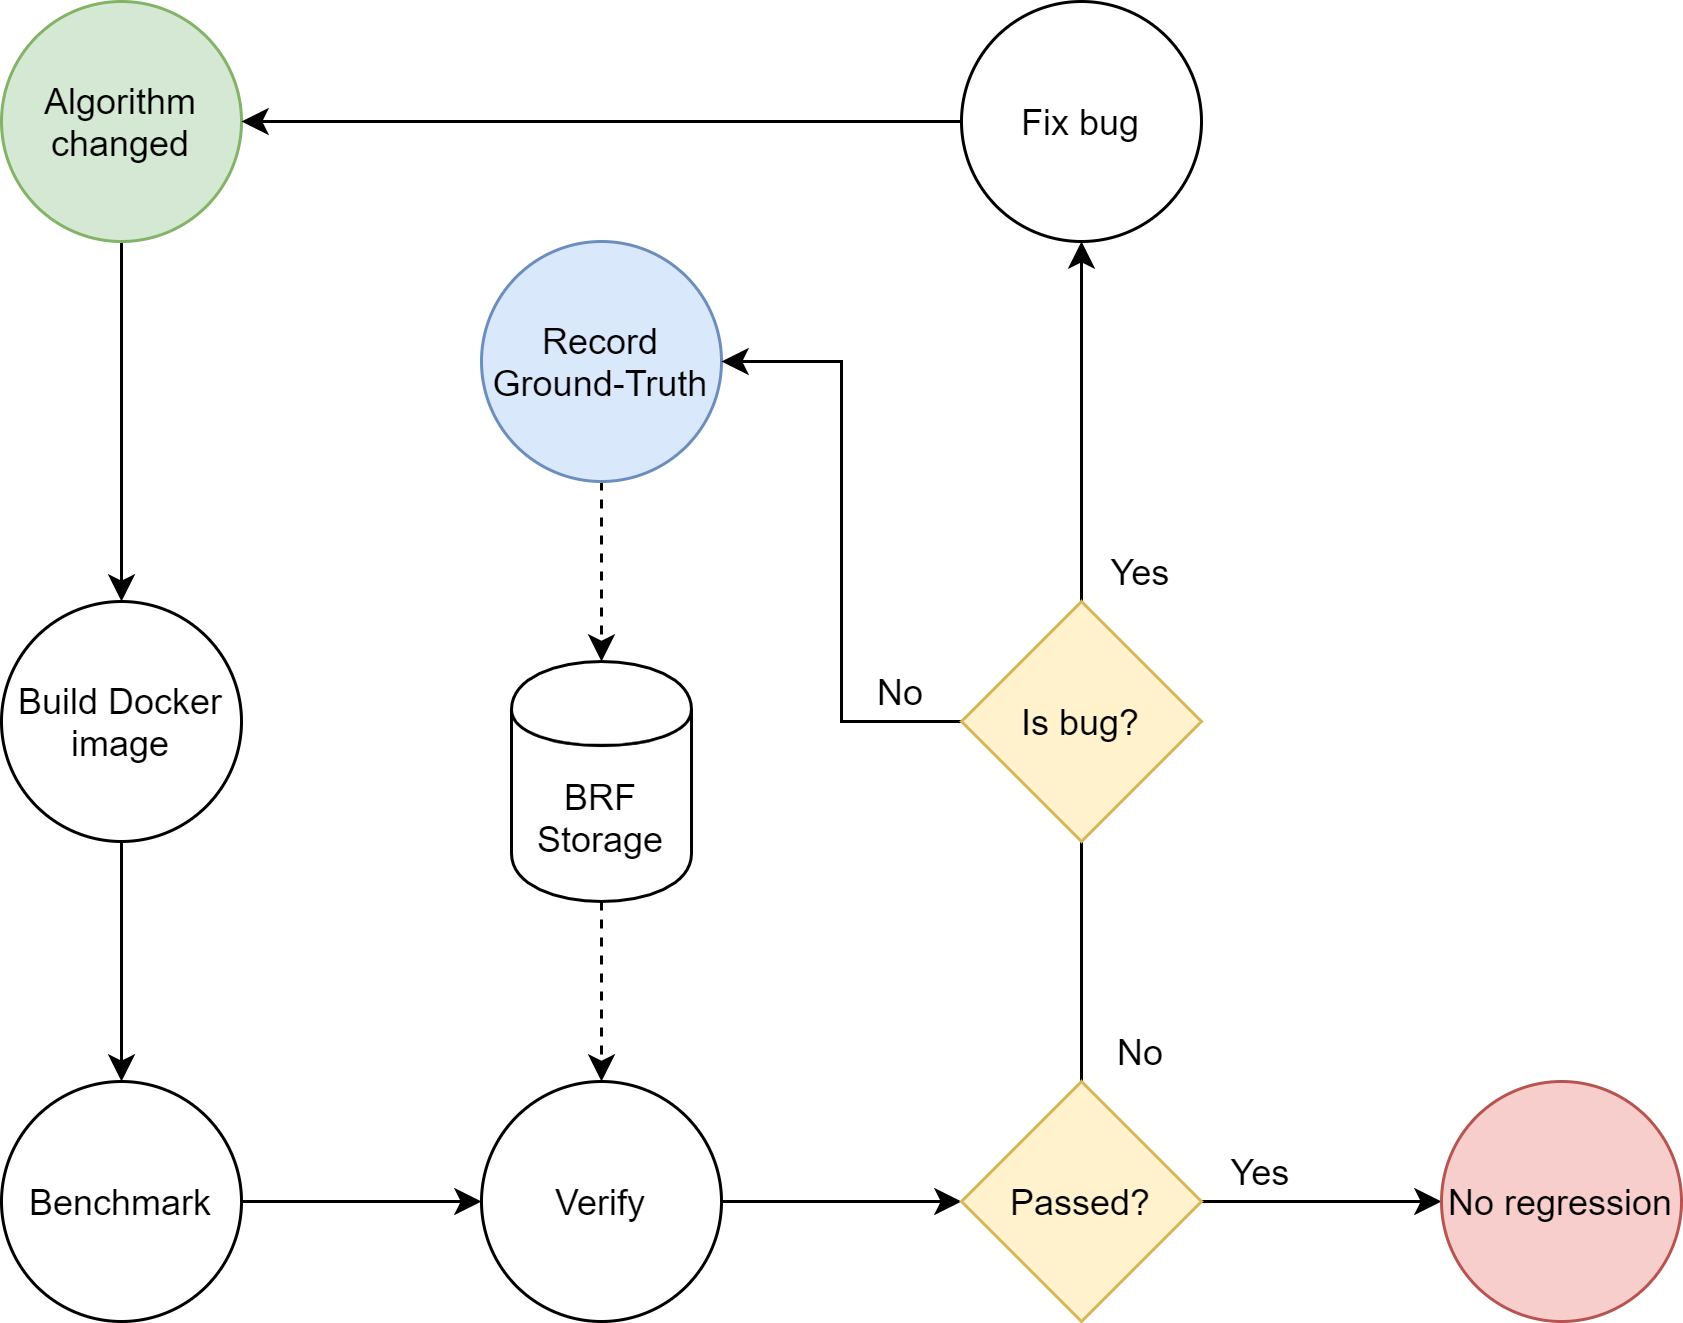
\includegraphics[width=\linewidth]{./img/crayon_for_regression_testing.png}
  \caption{Using Crayon benchmark and verify to protect against accuracy regressions. Initially a ground truth benchmark (in blue) need to be recorded. Therafter, whenever a code change occurs (in green), the algorithm is tested with Crayon through the \textit{crayon.benchmark} \& \textit{crayon.verify} functions.}
  \label{fig:crayon_as_test}
\end{figure}

\subsection{Scope and Limitations}
Since the main goal of this thesis is to perform a emprical comparison of forecasting methods, the study made in this section is deliberately small scaled. It serves as a proof of concept of how a benchmarking tool such as Crayon can be applied to other domains such as automated testing during development of time series forecasing algorithms. Furthermore, since executing all of the 400 training jobs required for a complete benchmark removes valuable time from the empirical comparison, the datasets used were the \textit{electricity} and the \textit{m4\_daily}.

\subsection{Methodology}
To evaluate Crayon for catching accuracy regressions, three Docker images of Gluon-TS is required. One image containing the code before the regression occured, the second image contains the version of Gluon-TS where the DeepAREstimator suffered an accuracy regression. The third image contains the version of Gluon-TS where the issue was fixed. These three images are hereby referred to as \textit{ground-truth image}, \textit{bugged image} and \textit{post-fix image}. Benchmarks using these three images are then performed and the generated BRFs are stored. Then each benchmark is verified against all other benchmarks with the results summarized into a table. All Docker images are then pushed to the public Dockerhub repository \textit{arangatang/masterthesis} \cite{dockerhub_arangatang}.


\subsection{Result}
In Table \ref{tab:crayon_for_accuracy_regressions} the results from the study are presented. The results show that the accuracy regression is successfully detected by the KS test for each metric since the verification passes 0 out of 3 times when comparing the \textit{pre-bug} image with the \textit{bugged} image across all metrics. Figure \ref{fig:crayon_as_test_deepar_all_rmse_solar} shows violin plots of the RMSE distributions for the three images on the \textit{Solar Energy} dataset. This plot shows that the change in distribution for the RMSE distribution between the bugged and the other images is substantial. Thus it makes sense that the KS test detected this, however, in this scenario a simpler test such as the naive approach investigated in Section \ref{sec:compairing_hypothesis_tests} should suffice.


\begin{table}[htb]
  \centering
  \begin{tabular}{cccc}
    DeepAR version & \rothalf{Pre-Bug}     & \rothalf{Bugged}     & \rothalf{Post-Fix}   \\ [0.5ex]
    \hline
    \multicolumn{4}{c}{\cellcolor{gray!25}MAPE}                                          \\
    \hline
    Pre-Bug        & \cellcolor{green}3/3  & -                    & -                    \\
    Bugged         & \cellcolor{green}0/3  & \cellcolor{green}3/3 & -                    \\
    Post-Fix       & \cellcolor{green}3/3  & \cellcolor{green}0/3 & \cellcolor{green}3/3 \\
    \multicolumn{4}{c}{\cellcolor{gray!25}MASE}                                          \\
    \hline
    Pre-Bug        & \cellcolor{green}3/3  & -                    & -                    \\
    Bugged         & \cellcolor{green}0/3  & \cellcolor{green}3/3 & -                    \\
    Post-Fix       & \cellcolor{orange}1/3 & \cellcolor{green}0/3 & \cellcolor{green}3/3 \\
    \multicolumn{4}{c}{\cellcolor{gray!25}Absolute Error}                                \\
    \hline
    Pre-Bug        & \cellcolor{green}3/3  & -                    & -                    \\
    Bugged         & \cellcolor{green}0/3  & \cellcolor{green}3/3 & -                    \\
    Post-Fix       & \cellcolor{green}3/3  & \cellcolor{green}0/3 & \cellcolor{green}3/3 \\
    \multicolumn{4}{c}{\cellcolor{gray!25}RMSE}                                          \\
    \hline
    Pre-Bug        & \cellcolor{green}3/3  & -                    & -                    \\
    Bugged         & \cellcolor{green}0/3  & \cellcolor{green}3/3 & -                    \\
    Post-Fix       & \cellcolor{orange}1/3 & \cellcolor{green}0/3 & \cellcolor{green}3/3 \\
    \multicolumn{4}{c}{\cellcolor{gray!25}MSIS}                                          \\
    \hline
    Pre-Bug        & \cellcolor{green}3/3  & -                    & -                    \\
    Bugged         & \cellcolor{green}0/3  & \cellcolor{green}3/3 & -                    \\
    Post-Fix       & \cellcolor{orange}1/3 & \cellcolor{green}0/3 & \cellcolor{green}3/3 \\
    \hline
  \end{tabular}
  \caption{Number of successfull benchmark verifications for three versions of DeepAR, two without bugs, one with. The benchmarks ran on the \textit{Electricity}, \textit{Solar Energy} and \textit{M4 Daily} datasets and error metric distributions were collected for five different error metrics on each. Optimal results marked in Green, partially optimal results are shown in Orange.}
  \label{tab:crayon_for_accuracy_regressions}
\end{table}

\begin{figure}[h]
  \centering
  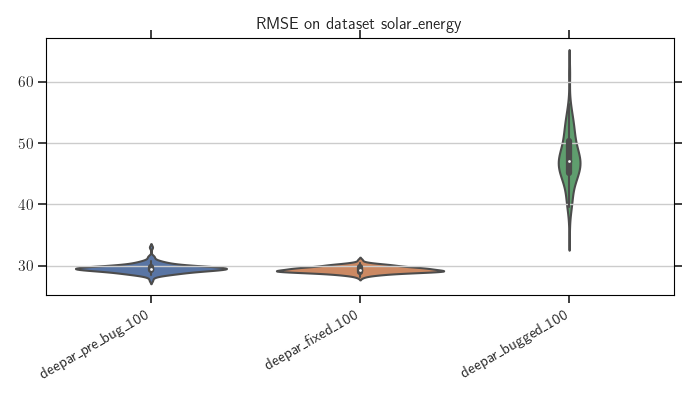
\includegraphics[width=\linewidth]{./img/crayon_study/RMSE_all_solar.png}
  \caption{Violin plots of the RMSE error distributions for the three versions of DeepAR on the solar dataset.}
  \label{fig:crayon_as_test_deepar_all_rmse_solar}
\end{figure}

The data in Table \ref{tab:crayon_for_accuracy_regressions} also shows that the \textit{bugged} image fails verification with the \textit{post-fix} image which is expected as the bug should be resolved. However, comparing the \textit{post-fix} image with the \textit{pre-bug} image fails on the \textit{M4 Daily} and the \textit{Solar Energy} datasets. This means that either the performance of DeepAR changed over the course of the 2 months between the patch or that the samples used were too few so that the KS test was unstable.

To investigate this, violin plots of the \textit{pre-bug} and the \textit{post-fix} error distributions were generated. In Figure \ref{fig:crayon_as_test_deepar_prepost_solar} two of these are presented, one for the MSIS error metric and one for the RMSE error metrics. From these, it seems that the MSIS distribution changed during the two months that the bug was present. Furthermore, it makes sense that the KS metric classified the \textit{pre-bug} metric and the \textit{post-fix} distributions as being sampled from different populations since the mean and variance of the samples differ substantially. However for the RMSE violin plots the difference is not as clear cut.

In total there were 43 commits added to Gluon-TS in the two months when the accuracy regression happened \cite{gluonts-github}. Three of them are possible causes of the detected change in accuracy between the \textit{pre-bug} and \textit{post-fix} versions. The first of these enabled multiprocessing for backtesting, as discussed in Section \ref{subsec:sources_randomness} multiprocessing can introduce additional data shuffling which can affect performance. The second change was to how the Negative Binomial was calculated and the third was a change to how MSIS error metrics was calculated. All three of these changes has immediate effect on the error distributions being tested, thus, this indicates that a second accuracy change occurred and that the KS test did not become unstable. Further investigation is needed to verify this further, however due to the time consuming process of benchmarking deepar multiple times more, this is left for future work.

To summarize, the results show that the KS test successfully identified the accuracy regression introduced on the 7th of May. Furthermore, it may have identified a second accuracy change introduced during the time the investigated bug was unnoticed. This result indicates that the benchmark and verification systems in Crayon are suitable for detecting accuracy regressions during development of time series forecasting models in time series forecasting frameworks such as Gluon-TS.

% \begin{figure}[h]
%   \centering
%   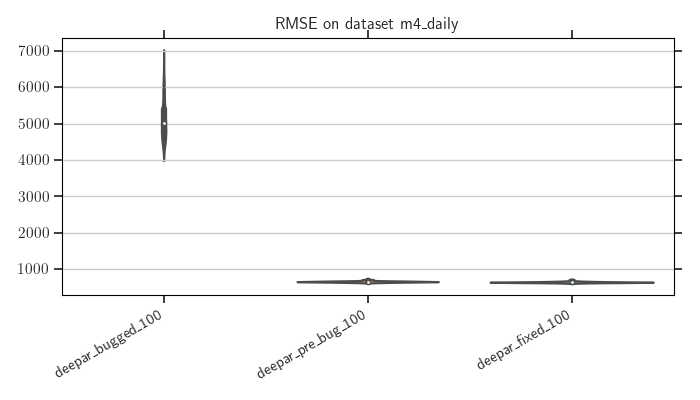
\includegraphics[width=\linewidth]{./img/crayon_study/RMSE_all_m4.png}
%   \caption{Violin plots of the RMSE error distributions for the three versions of DeepAR on the M4 dataset.}
%   \label{fig:crayon_as_test_deepar_rmse_all_m4}
% \end{figure}



% \begin{figure}[h]
% \centering
%   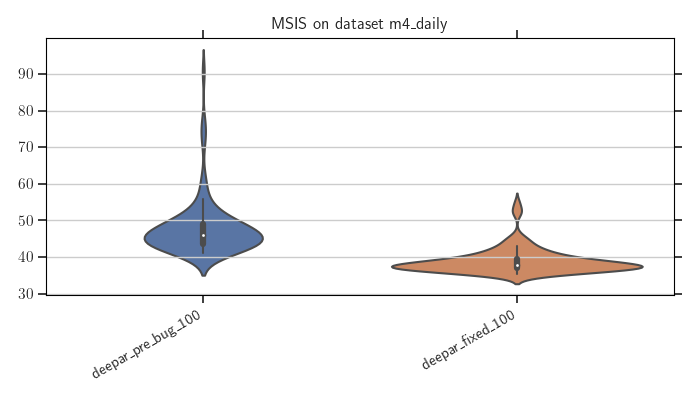
\includegraphics[width=\linewidth]{./img/crayon_study/MSIS_pre_and_fixed_m4.png}
%   \caption{Violin plots of the RMSE error distributions for the three versions of DeepAR on the solar dataset.}
%   \label{fig:crayon_as_test_deepar_prepost_msis_m4}
% \end{figure}


% \begin{figure}[h]
%   \centering
%   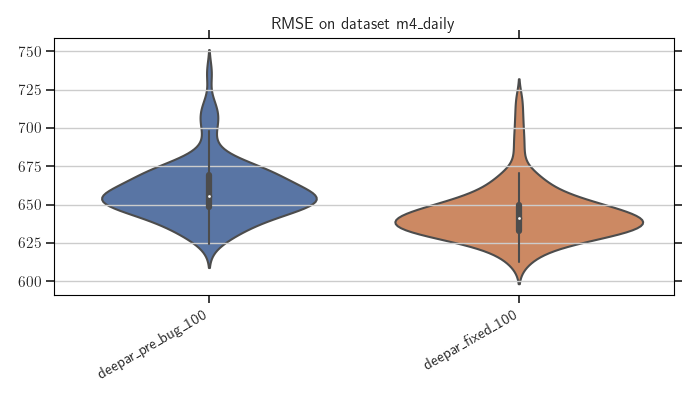
\includegraphics[width=\linewidth]{./img/crayon_study/RMSE_pre_and_fix_m4.png}
%   \caption{Violin plots of the RMSE error distributions for the three versions of DeepAR on the solar dataset.}
%   \label{fig:crayon_as_test_deepar_prepost_rmse_m4}
% \end{figure}
\begin{figure}[ht]
  \centering
  \begin{minipage}[b]{0.95\linewidth}
    \centering
    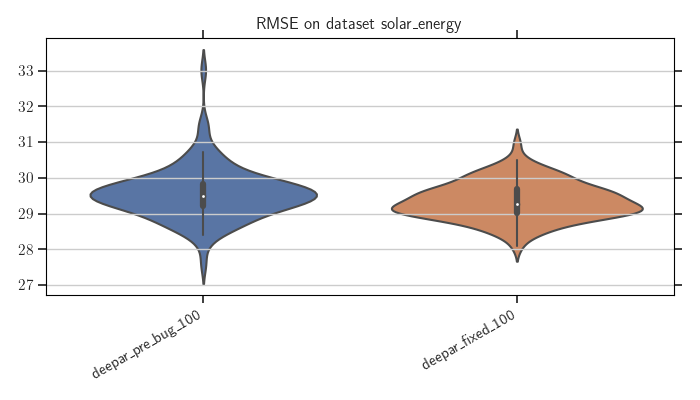
\includegraphics[width=\linewidth]{./img/crayon_study/RMSE_pre_and_fixed_solar.png}
    % \vspace{4ex}
  \end{minipage}%% 

  \begin{minipage}[b]{0.95\linewidth}
    \centering
    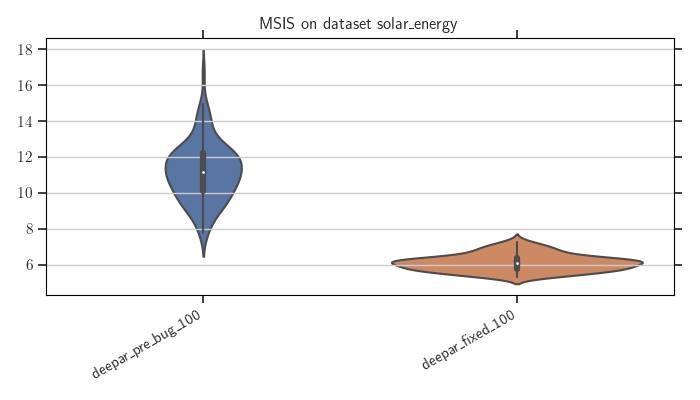
\includegraphics[width=\linewidth]{./img/crayon_study/MSIS_pre_and_fixed_solar.png}
    % \vspace{4ex}
  \end{minipage}
  \caption{Violin plots of the RMSE and MSIS error distributions on the solar dataset for the \textit{fixed} and \textit{pre-bug} versions of DeepAR.}
  \label{fig:crayon_as_test_deepar_prepost_solar}
\end{figure}
% \begin{figure}[h]
%   \centering
%   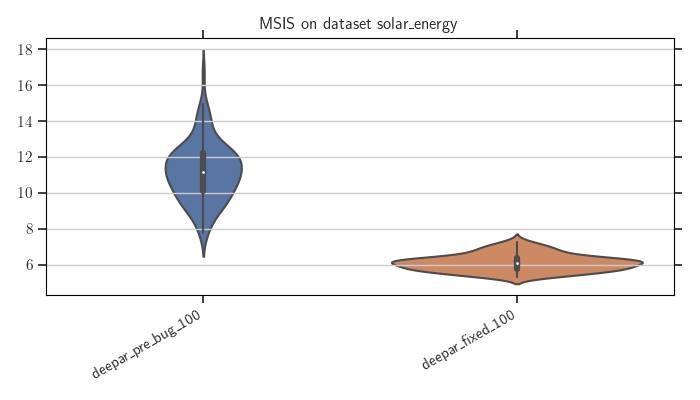
\includegraphics[width=\linewidth]{./img/crayon_study/MSIS_pre_and_fixed_solar.png}
%   \caption{Violin plots of the RMSE error distributions for the three versions of DeepAR on the solar dataset.}
%   \label{fig:crayon_as_test_deepar_prepost_msis_solar}
% \end{figure}

% \begin{figure}[h]
%   \centering
%   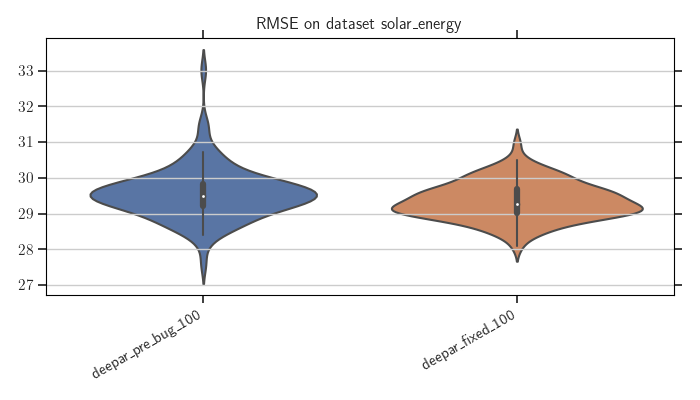
\includegraphics[width=\linewidth]{./img/crayon_study/RMSE_pre_and_fixed_solar.png}
%   \caption{Violin plots of the RMSE error distributions for the three versions of DeepAR on the solar dataset.}
%   \label{fig:crayon_as_test_deepar_prepost_rmse_solar}
% \end{figure}
